\documentclass[11pt,a4paper]{article}

\usepackage[margin=1in]{geometry}
\usepackage{graphicx}
\usepackage{booktabs}
\usepackage{array}
\usepackage{float}
\usepackage{url}
\usepackage{amsmath}
\usepackage{tikz}
\usetikzlibrary{positioning,arrows.meta}
\usepackage[hidelinks]{hyperref}

\graphicspath{{figures/}}

\title{\textbf{SentiBias Audit}\\[4pt]
\large Auditing Multilingual Sentiment Models for Dialect, Gender and Code-Switching Bias\\[6pt]
\normalsize AI Project --- Deliverable 2: Model Architecture \& Empirical Evaluation}
\author{Saad Jahangir \and Talmeez ur Rehman \and Muhammad Yaseen Asif}
\date{November 2026}

\begin{document}
\maketitle

\begin{abstract}
This deliverable builds and evaluates the sentiment models that SentiBias Audit audits.
A frozen multilingual transformer (MiniLM-L12) produces sentence embeddings, and a PyTorch
multi-layer perceptron trained on top of them classifies Roman Urdu and English text as
negative, neutral or positive. The model is compared with a TF-IDF + Logistic Regression
baseline in scikit-learn. A stratified 70/15/15 split, a 24-configuration hyperparameter search
and a held-out test set give a test macro-F1 of 0.638 and macro AUC-ROC of 0.828, against 0.616 / 0.806 for the
baseline. The error analysis and Bias Check show a clear language gap (macro-F1 0.67 on
English vs.\ 0.54 on Roman Urdu) and statistically significant but small gender score gaps on
the Equity Evaluation Corpus, in opposite directions for the two models. All code is in
\texttt{src/}.
\end{abstract}

% ---------------------------------------------------------------------------
\section{Recap of Deliverable 1}
Deliverable~1 collected three datasets (UCI Roman Urdu, TweetEval sentiment, Equity Evaluation
Corpus), cleaned them into an 87,696-row master file with a unified schema (text, label,
language, source, gender, code-switching flag and length features), and built normalised text, encoded labels (negative = 0, neutral = 1, positive = 2) and a TF-IDF
representation (\path{data_scripts/}). Deliverable~2 starts from these processed files.

% ---------------------------------------------------------------------------
\section{Phase 3: Model Architecture \& Implementation}

\subsection{Framework Selection}
\begin{itemize}
  \item \textbf{PyTorch} (\texttt{torch}~2.x) for the main neural model: layers, loss,
        optimizer and the training loop are written by hand in \path{src/model.py} and
        \path{src/train.py}.
  \item \textbf{sentence-transformers} (on top of Hugging Face \texttt{transformers}) to load the
        pre-trained multilingual encoder \texttt{paraphrase-multilingual-MiniLM-L12-v2}
        (Reimers \& Gurevych, 2020), trained on 50+ languages including Urdu.
  \item \textbf{scikit-learn} for the baseline (TF-IDF + Logistic Regression), the data split
        and all metrics.
\end{itemize}
The encoder is \emph{frozen}: all 87,696 sentences are embedded once (\path{src/embed.py}, 23
minutes on a 12-core CPU, no GPU available) and only the classification head is trained. This
keeps training to about 3~seconds per epoch, which made a full hyperparameter grid possible
on a laptop. It also matches the audit goal: we measure the bias of a widely used pre-trained
multilingual encoder, not of weights we changed ourselves. Full fine-tuning of the encoder is
left for the mitigation phase.

\subsection{Design: Layers, Loss and Optimizer}

\begin{figure}[H]
\centering
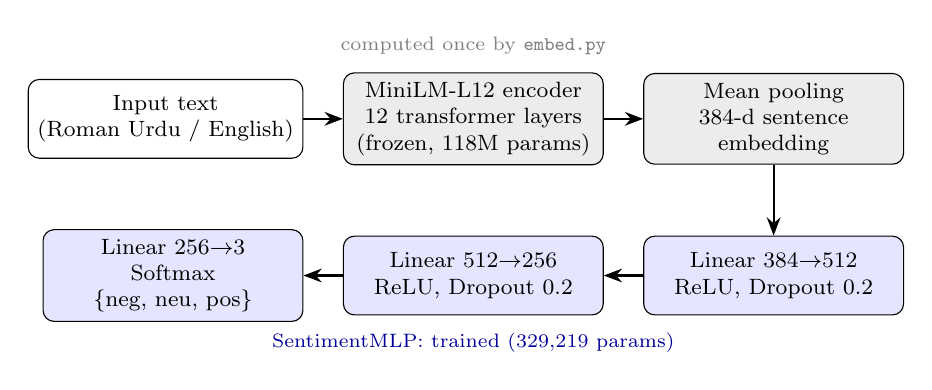
\begin{tikzpicture}[
  node distance=5mm,
  box/.style={draw, rounded corners, align=center, minimum width=3.3cm, minimum height=10mm, font=\footnotesize},
  frozen/.style={box, fill=gray!15},
  train/.style={box, fill=blue!10},
  arr/.style={-{Stealth}, thick}]
\node[box] (in) {Input text\\(Roman Urdu / English)};
\node[frozen, right=of in] (enc) {MiniLM-L12 encoder\\12 transformer layers\\(frozen, 118M params)};
\node[frozen, right=of enc] (pool) {Mean pooling\\384-d sentence\\embedding};
\node[train, below=9mm of pool] (l1) {Linear 384$\to$512\\ReLU, Dropout 0.2};
\node[train, left=of l1] (l2) {Linear 512$\to$256\\ReLU, Dropout 0.2};
\node[train, left=of l2] (l3) {Linear 256$\to$3\\Softmax\\\{neg, neu, pos\}};
\draw[arr] (in) -- (enc); \draw[arr] (enc) -- (pool); \draw[arr] (pool) -- (l1);
\draw[arr] (l1) -- (l2); \draw[arr] (l2) -- (l3);
\node[font=\scriptsize, gray, above=1mm of enc] {computed once by \texttt{embed.py}};
\node[font=\scriptsize, blue!60!black, below=1mm of l2] {SentimentMLP: trained (329,219 params)};
\end{tikzpicture}
\caption{Architecture of the main model. Grey blocks are the frozen pre-trained encoder; blue
blocks are the trainable classification head \texttt{SentimentMLP} (sizes shown are the final
tuned values $h = 512$, $p = 0.2$).}
\label{fig:arch}
\end{figure}

\paragraph{Layers.} \texttt{SentimentMLP} (\path{src/model.py}) is a two-hidden-layer
perceptron: $\text{Linear}(384, h) \to \text{ReLU} \to \text{Dropout}(p) \to
\text{Linear}(h, h/2) \to \text{ReLU} \to \text{Dropout}(p) \to \text{Linear}(h/2, 3)$.
The output is three logits; the softmax is applied inside the loss during training and
explicitly at prediction time.

\paragraph{Loss function.} The labelled data is imbalanced (neutral 45\%, positive 34\%,
negative 21\% of the training split), so plain cross-entropy would favour the neutral class.
We use class-weighted cross-entropy
\[
\mathcal{L} = -\frac{1}{N}\sum_{i} w_{y_i}\log \operatorname{softmax}(z_i)_{y_i},\qquad
w_c = \frac{N}{3\,N_c},
\]
which gives $w_{\text{neg}} = 1.60$, $w_{\text{neu}} = 0.73$, $w_{\text{pos}} = 0.99$ on the
training split.

\paragraph{Optimizer.} AdamW (Adam with decoupled weight decay $10^{-4}$), mini-batch training
with shuffling, at most 40 epochs, and early stopping on validation macro-F1 with patience~4.
The weights of the best epoch are restored.

\paragraph{Baseline.} \path{src/baseline.py} uses the same TF-IDF settings as Deliverable~1
(unigrams + bigrams, 5,000 features, \texttt{min\_df}=2) followed by multinomial Logistic
Regression with balanced class weights (L-BFGS solver, L2 penalty). The TF-IDF vocabulary is
now fitted on the training split only; in Deliverable~1 it was fitted on all rows, which would
leak test vocabulary into training.

\subsection{Hyperparameter Tuning}
\path{src/tune.py} runs a full grid search of $3 \times 2 \times 2 \times 2 = 24$ configurations.
Each one is trained on the training split with early stopping (max.\ 25 epochs) and scored
by macro-F1 on the validation split. The test split is not used for tuning.
Table~\ref{tab:grid} lists the values tested and Table~\ref{tab:tuning} the results.

\begin{table}[H]
\centering
\small
\begin{tabular}{lll}
\toprule
\textbf{Hyperparameter} & \textbf{Values tested} & \textbf{Selected} \\
\midrule
Learning rate (AdamW) & $10^{-2}$, $10^{-3}$, $10^{-4}$ & $10^{-4}$ \\
Batch size            & 64, 256                         & 64 \\
Dropout $p$           & 0.2, 0.5                        & 0.2 \\
Hidden size $h$       & 256, 512                        & 512 \\
Weight decay          & $10^{-4}$ (fixed)               & $10^{-4}$ \\
Epochs                & early stopping, patience 4      & 11 (best epoch) \\
\midrule
Baseline: LogReg $C$  & 0.1, 0.3, 1, 3, 10              & 1 \\
\bottomrule
\end{tabular}
\caption{Hyperparameter search space and final selection.}
\label{tab:grid}
\end{table}

\begin{table}[H]
\centering
\small
\begin{tabular}{rrrrrrr}
\toprule
\textbf{LR} & \textbf{Batch} & \textbf{Dropout} & \textbf{Hidden} & \textbf{Best epoch} & \textbf{Val acc.} & \textbf{Val macro-F1} \\
\midrule
$10^{-4}$ & 64  & 0.2 & 512 & 11 & 0.652 & \textbf{0.646} \\
$10^{-4}$ & 256 & 0.2 & 512 & 21 & 0.650 & 0.645 \\
$10^{-4}$ & 64  & 0.5 & 512 & 16 & 0.649 & 0.644 \\
$10^{-4}$ & 64  & 0.5 & 256 & 24 & 0.645 & 0.642 \\
$10^{-3}$ & 256 & 0.5 & 512 & 8  & 0.645 & 0.642 \\
$10^{-3}$ & 256 & 0.2 & 256 & 7  & 0.644 & 0.640 \\
$10^{-3}$ & 64  & 0.2 & 512 & 3  & 0.637 & 0.634 \\
$10^{-2}$ & 256 & 0.2 & 256 & 11 & 0.633 & 0.630 \\
$10^{-2}$ & 64  & 0.2 & 256 & 5  & 0.603 & 0.603 \\
$10^{-2}$ & 64  & 0.5 & 512 & 1  & 0.503 & 0.501 \\
\bottomrule
\end{tabular}
\caption{Selected rows of the 24-run grid (full table: \texttt{results/tuning\_results.csv}).
Baseline $C$ search: val macro-F1 0.601 / 0.615 / \textbf{0.618} / 0.612 / 0.606 for
$C$ = 0.1 / 0.3 / 1 / 3 / 10.}
\label{tab:tuning}
\end{table}

\paragraph{Justification.}
\begin{itemize}
  \item \textbf{Learning rate} is the most important hyperparameter. With $10^{-2}$ training is
        unstable: in two runs the best epoch is epoch~1, and the worst run reaches only 0.50
        macro-F1.
        $10^{-3}$ converges in 3--11 epochs but starts to overfit early. $10^{-4}$ gives
        the best 4 of 24 runs, because the smaller steps reach a better minimum.
  \item \textbf{Batch size} 64 is slightly better than 256 at the same learning rate (0.646 vs.\
        0.645). It needs half as many epochs (11 vs.\ 21), so it was selected.
  \item \textbf{Dropout} 0.2 is better than 0.5 for the larger head. The input is already a
        compact, pre-trained 384-d embedding, so strong dropout removes useful signal.
        Overfitting is controlled by early stopping instead.
  \item \textbf{Hidden size} 512 is better than 256 in every learning-rate/dropout pair at
        $10^{-4}$. The extra capacity helps the head separate the two languages, which share
        one embedding space.
\end{itemize}
The final model was retrained with the selected values (\path{src/train.py}) and reproduced the
tuning score exactly (0.6462), so the run is deterministic with the fixed seed 42.

% ---------------------------------------------------------------------------
\section{Phase 4: Training \& Evaluation}

\subsection{Validation Strategy}
\path{src/split_data.py} creates one fixed, \textbf{stratified 70/15/15
train/validation/test split} of the two labelled corpora. The strata are
\emph{language $\times$ label}, so every split has the same language mix and class balance
(Table~\ref{tab:split}). The original TweetEval split was not reused: its validation set is
only 2,000 tweets (3\%) and it does not cover Roman Urdu. The \textbf{EEC is never used for
training}. All 8,640 EEC sentences form a separate ``bias'' split used only for the Bias
Check. The validation split is used for early stopping and tuning, and the test split is used
once, for the final numbers below.

\begin{table}[H]
\centering
\small
\begin{tabular}{llrrrr}
\toprule
\textbf{Split} & \textbf{Language} & \textbf{Negative} & \textbf{Neutral} & \textbf{Positive} & \textbf{Total} \\
\midrule
Train (70\%) & English    & 7,962 & 19,222 & 14,724 & 41,908 \\
             & Roman Urdu & 3,560 & 5,908  & 3,963  & 13,431 \\
Val (15\%)   & English    & 1,706 & 4,119  & 3,155  & 8,980 \\
             & Roman Urdu & 763   & 1,266  & 849    & 2,878 \\
Test (15\%)  & English    & 1,707 & 4,119  & 3,155  & 8,981 \\
             & Roman Urdu & 763   & 1,266  & 849    & 2,878 \\
\midrule
Bias (EEC)   & English    & 6,300 & 240    & 2,100  & 8,640 \\
\bottomrule
\end{tabular}
\caption{Rows per split. Train/val/test contain 55,339 / 11,858 / 11,859 rows.}
\label{tab:split}
\end{table}

\subsection{Training Curves}
\begin{figure}[H]
\centering
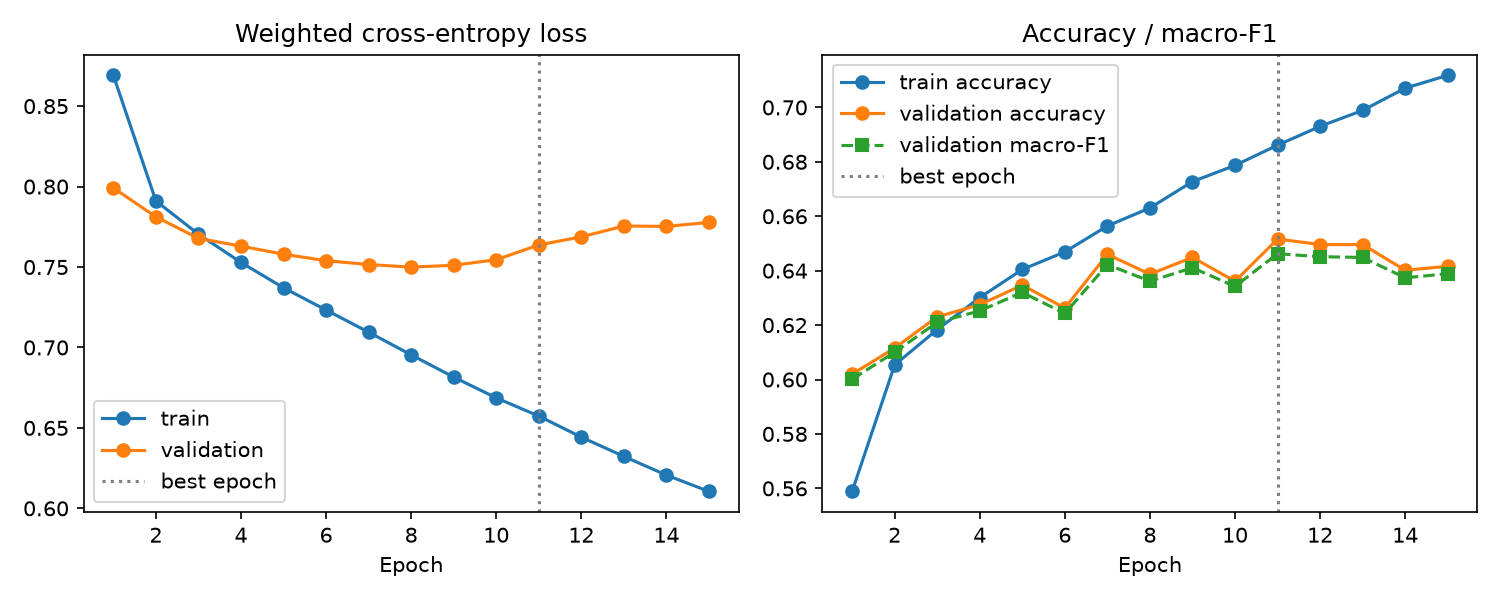
\includegraphics[width=0.95\textwidth]{training_curves.png}
\caption{Loss and accuracy of the final model. Training loss keeps falling, but validation
loss is lowest at epoch~8 and validation macro-F1 peaks at epoch~11, after which the model
overfits. Early stopping ended training at epoch~15 and restored the epoch-11 weights.}
\label{fig:curves}
\end{figure}

\subsection{Metric Analysis}

\begin{table}[H]
\centering
\small
\begin{tabular}{lrrrrr}
\toprule
\textbf{Model} & \textbf{Accuracy} & \textbf{Macro-P} & \textbf{Macro-R} & \textbf{Macro-F1} & \textbf{Macro AUC-ROC} \\
\midrule
TF-IDF + LogReg (baseline) & 0.621 & 0.612 & 0.633 & 0.616 & 0.806 \\
MiniLM + MLP (ours)        & \textbf{0.643} & \textbf{0.633} & \textbf{0.652} & \textbf{0.638} & \textbf{0.828} \\
\bottomrule
\end{tabular}
\caption{Results on the held-out test split (11,859 rows). AUC-ROC is one-vs-rest, macro-averaged.}
\label{tab:test}
\end{table}

\begin{table}[H]
\centering
\small
\begin{tabular}{lrrrrrrr}
\toprule
 & & \multicolumn{3}{c}{\textbf{TF-IDF + LogReg}} & \multicolumn{3}{c}{\textbf{MiniLM + MLP}} \\
\cmidrule(lr){3-5}\cmidrule(lr){6-8}
\textbf{Class} & \textbf{Support} & P & R & F1 & P & R & F1 \\
\midrule
Negative & 2,470 & 0.487 & 0.673 & 0.565 & 0.524 & 0.690 & 0.595 \\
Neutral  & 5,385 & 0.686 & 0.571 & 0.623 & 0.690 & 0.612 & 0.649 \\
Positive & 4,004 & 0.663 & 0.657 & 0.660 & 0.684 & 0.655 & 0.669 \\
\bottomrule
\end{tabular}
\caption{Per-class precision, recall and F1 on the test split.}
\label{tab:perclass}
\end{table}

\paragraph{Why these metrics.}
\begin{itemize}
  \item \textbf{Macro-F1 is the main metric} (used for model selection and early stopping). The
        classes are imbalanced: negative is only 21\% of the test set, while neutral is 45\%.
        Accuracy and micro-averaged scores are dominated by the neutral class. Macro-averaging
        gives each class equal weight, so a model cannot score well by ignoring negative text,
        which matters most for content moderation.
  \item \textbf{Precision and recall} are reported separately because the two kinds of error
        cost different things. Low negative precision (0.52) means many neutral posts get
        flagged as negative (false alarms). Recall shows how many truly negative posts are
        caught. The class weights deliberately trade some negative precision for higher
        negative recall (0.69).
  \item \textbf{AUC-ROC} measures ranking quality across all thresholds and does not depend
        on class priors. That matters here because EEC and the two training corpora have very
        different label distributions. The bias check also uses the model's probabilities, not
        only its labels, so ranking quality is relevant.
  \item \textbf{Accuracy} is reported for completeness, but it is not used to choose models.
\end{itemize}

\begin{figure}[H]
\centering
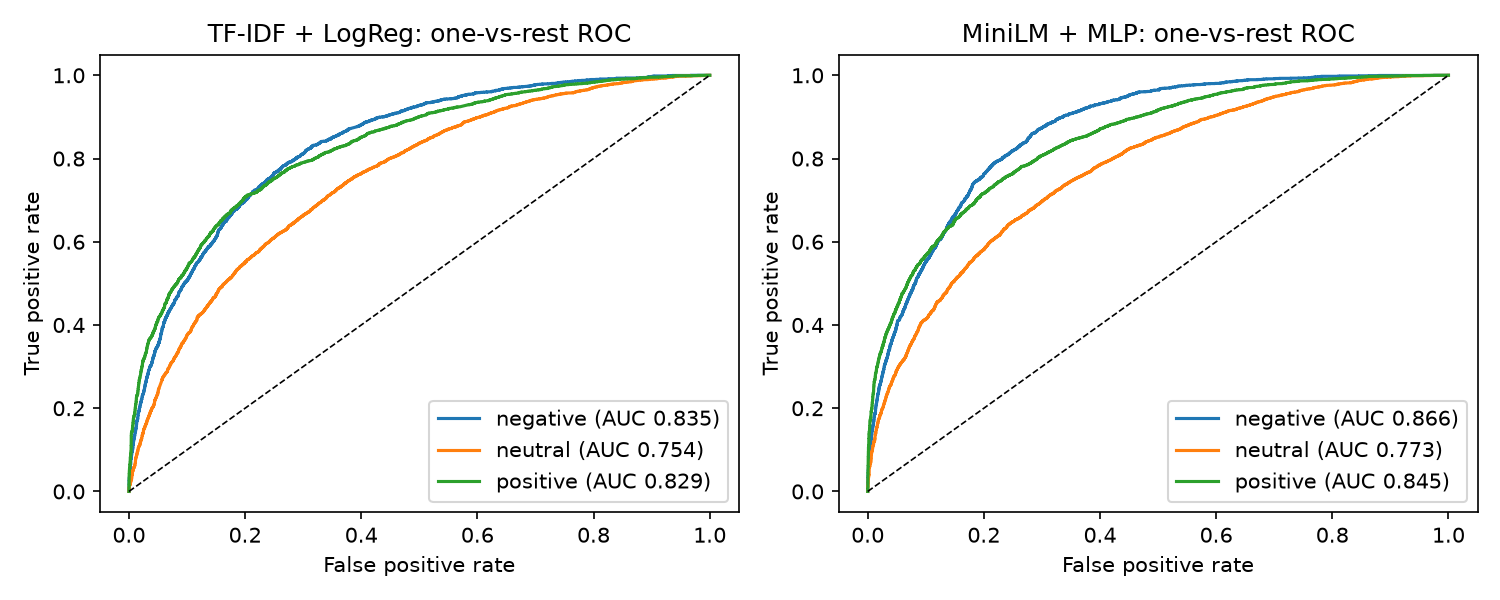
\includegraphics[width=0.95\textwidth]{roc_curves.png}
\caption{One-vs-rest ROC curves on the test split. Neutral is the hardest class for both
models (AUC 0.75--0.77).}
\label{fig:roc}
\end{figure}

\subsection{Error Analysis}

\begin{figure}[H]
\centering
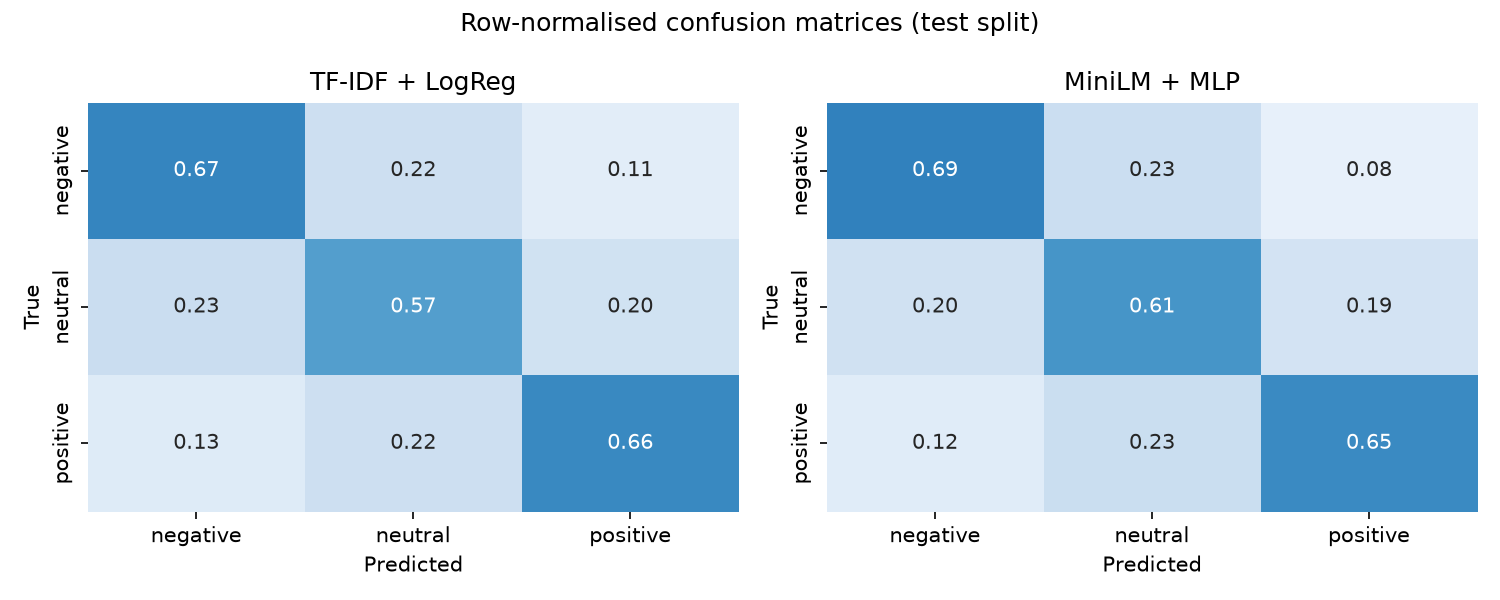
\includegraphics[width=0.9\textwidth]{confusion_matrices.png}
\caption{Row-normalised confusion matrices on the test split.}
\label{fig:cm}
\end{figure}

\paragraph{Which classes fail.} Neutral is the weakest class. For the MLP, the four most
frequent error types all involve neutral: neutral$\to$negative (1,088), neutral$\to$positive
(1,004), positive$\to$neutral (919) and negative$\to$neutral (559). Direct polarity swaps are
rarer (positive$\to$negative 464, negative$\to$positive 206). Most errors are therefore about
\emph{how strong} the sentiment is, not \emph{which way} it points. Compared with the baseline,
the MLP mainly reduces neutral$\to$negative false alarms (1,247 $\to$ 1,088).

\paragraph{Which inputs fail.} The most confident mistakes (\path{results/error_examples.csv})
fall into four groups:
\begin{enumerate}
  \item \emph{Label noise in Roman Urdu}: ``She is awesome'' and ``I watched really enjoyed it''
        are labelled neutral, and the model predicts positive with 99\% confidence. The UCI
        labels are sometimes inconsistent, which puts a ceiling on achievable Roman Urdu scores.
  \item \emph{Mixed sentiment in one post}: ``product is amazing \ldots\ lkn bazar ke lehaz se price
        zyada hai'' (\emph{but the price is high compared with the market}) praises and
        complains in one sentence. The complaint is the Roman Urdu half, which both models
        miss.
  \item \emph{Sarcasm and political context} in tweets (``\#ThankYouObama for creating the
        strongest @user \ldots'' labelled negative), which needs world knowledge.
  \item \emph{Out-of-vocabulary words for the baseline}: only 11 of the 40 EEC emotion words
        (e.g.\ \emph{angry}, \emph{terrified}, \emph{horrible} are missing) are in the
        baseline's 5,000-term vocabulary. On EEC it therefore predicts mostly neutral and gets
        only 36.4\% accuracy, against 93.0\% for the MLP, whose subword tokenizer has no
        fixed vocabulary.
\end{enumerate}

\subsection{Bias Check}
The Bias Check covers the three dimensions defined in Deliverable~1: language variety,
code-switching, and gender / race-coded names.

\paragraph{1. Language (dialect) gap.} Figure~\ref{fig:subgroups} and Table~\ref{tab:lang} split
the test results by language. Both models are clearly worse on Roman Urdu. The transformer
model has the \emph{largest} gap: it gains 4 points of macro-F1 over the baseline on English
(0.671 vs.\ 0.629) but loses 4 points on Roman Urdu (0.535 vs.\ 0.573). Its English--Roman
Urdu gap is 0.136 macro-F1, more than twice the baseline's 0.056. The multilingual encoder was
pre-trained on Urdu in Arabic script, not on Latin-script Roman Urdu, so it does not
represent informal Roman Urdu well. A model that looks better overall is less fair to Roman
Urdu users, which is the hidden kind of gap that motivated this project.

\begin{table}[H]
\centering
\small
\begin{tabular}{lrrrrr}
\toprule
 & & \multicolumn{2}{c}{\textbf{TF-IDF + LogReg}} & \multicolumn{2}{c}{\textbf{MiniLM + MLP}} \\
\cmidrule(lr){3-4}\cmidrule(lr){5-6}
\textbf{Test subgroup} & \textbf{n} & Macro-F1 & AUC & Macro-F1 & AUC \\
\midrule
English (TweetEval)            & 8,981 & 0.629 & 0.816 & \textbf{0.671} & \textbf{0.854} \\
Roman Urdu (all)               & 2,878 & \textbf{0.573} & \textbf{0.770} & 0.535 & 0.723 \\
\quad code-switched            & 147   & \textbf{0.624} & \textbf{0.833} & 0.610 & 0.770 \\
\quad not code-switched        & 2,731 & \textbf{0.569} & \textbf{0.767} & 0.530 & 0.718 \\
\midrule
Gap English $-$ Roman Urdu     &       & 0.056 & 0.045 & 0.136 & 0.131 \\
\bottomrule
\end{tabular}
\caption{Test performance by language subgroup.}
\label{tab:lang}
\end{table}

\begin{figure}[H]
\centering
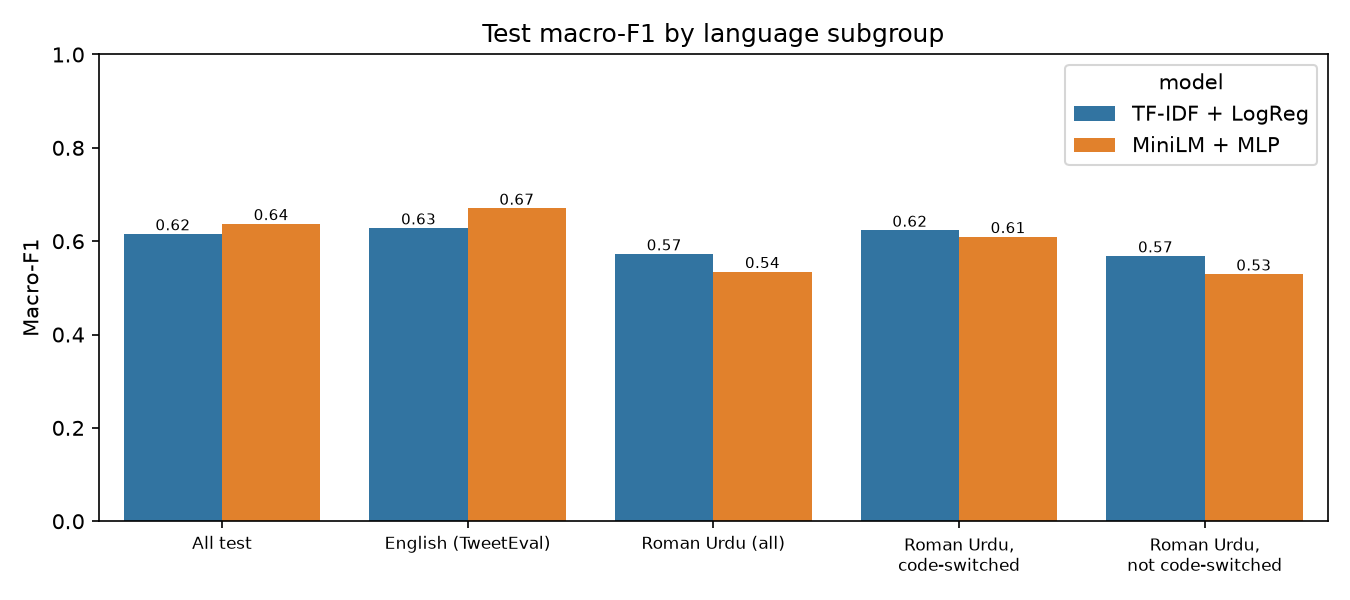
\includegraphics[width=0.9\textwidth]{subgroup_f1.png}
\caption{Test macro-F1 by language subgroup.}
\label{fig:subgroups}
\end{figure}

\paragraph{2. Code-switching.} Code-switched Roman Urdu--English posts score \emph{higher}
than monolingual Roman Urdu for both models (MLP: 0.610 vs.\ 0.530). The English words in
them (\emph{good, love, worst}) carry sentiment the models already know from TweetEval. This
group is small (147 test rows), so the estimate is noisy. Code-switching was also positively
correlated with the positive label in Deliverable~1 (6.4\% vs.\ 3.5\%), which makes these
posts easier. The problem is therefore pure Roman Urdu, not code-switching.

\paragraph{3. Gender and race (EEC).} For every EEC sentence we compute the sentiment score
$s = P(\text{positive}) - P(\text{negative})$. Sentences are grouped by (template, emotion
word), the mean score of female-name sentences is compared with male-name sentences in each
group, and a paired $t$-test is run over the 144 groups (Kiritchenko \& Mohammad, 2018). Race
uses only the name rows (African-American vs.\ European names). Results are in
Table~\ref{tab:bias} and Figure~\ref{fig:bias}.

\begin{table}[H]
\centering
\small
\begin{tabular}{llrrrr}
\toprule
\textbf{Model} & \textbf{Comparison} & \textbf{Mean gap} & \textbf{\% pairs A$>$B} & \textbf{$p$-value} & \textbf{Accuracy A / B} \\
\midrule
TF-IDF + LogReg & Female $-$ Male                 & $+0.070$ & 94.4\% & $5.8\times10^{-11}$ & 0.315 / 0.413 \\
                & Afr.-American $-$ European       & $+0.020$ & 97.2\% & $9.9\times10^{-42}$ & 0.281 / 0.351 \\
MiniLM + MLP    & Female $-$ Male                 & $-0.034$ & 9.7\%  & $6.4\times10^{-21}$ & 0.939 / 0.920 \\
                & Afr.-American $-$ European       & $-0.003$ & 62.5\% & 0.52 (n.s.)         & 0.917 / 0.931 \\
\bottomrule
\end{tabular}
\caption{EEC Bias Check over 144 (template, emotion word) pairs. A positive gap means group A
receives more positive sentiment. ``Accuracy A / B'' is the 3-class accuracy within each group.}
\label{tab:bias}
\end{table}

\begin{figure}[H]
\centering
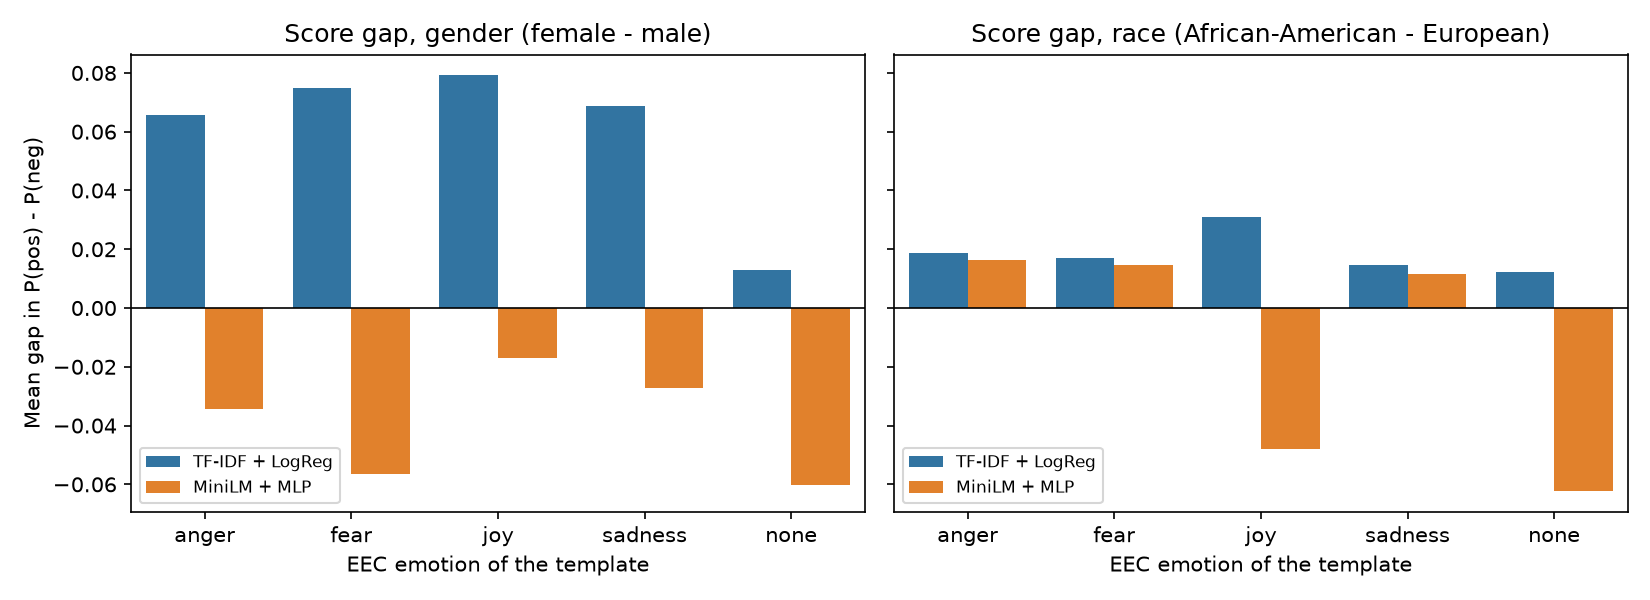
\includegraphics[width=0.98\textwidth]{bias_check.png}
\caption{Mean score gap per EEC emotion. The baseline rates female sentences more positively
for every emotion. The MLP rates them more negatively, most strongly for fear and for the
emotion-free (``none'') templates.}
\label{fig:bias}
\end{figure}

\noindent Findings:
\begin{itemize}
  \item \textbf{Both models show a statistically significant gender gap, in opposite
        directions.} The MLP gives the female version of a sentence a lower score in 90.3\%
        of pairs (mean $-0.034$). The gap is largest for fear ($-0.057$) and for neutral
        templates ($-0.060$), so sentences such as ``\emph{She} has two children'' are read
        as more negative than the male version. Since the encoder is frozen, this
        association comes from the pre-trained MiniLM embeddings.
  \item \textbf{The baseline's gap is explained by individual words it learned from tweets.}
        No female name and only two African-American names are in its vocabulary. Its gap
        therefore comes from noun phrases and pronouns with learned weights. For example, the
        positive-minus-negative weight is $+1.31$ for ``my mom'' vs.\ $0.00$ for ``my dad'' and
        $+0.60$ for ``her'' vs.\ $-0.40$ for ``him''. Several European male names (Adam,
        Roger) have strongly negative weights, probably from tweets about specific people.
        This shows how bias enters even a simple bag-of-words model through training data.
  \item \textbf{Race:} the MLP shows no significant overall race gap ($p = 0.52$), but its
        per-emotion gaps go both ways (Figure~\ref{fig:bias}): African-American names get a
        lower score on joy ($-0.048$) and neutral ($-0.062$) templates. The baseline's race gap
        is significant but small ($+0.020$).
  \item \textbf{Size of the effect.} The gender gaps (0.03--0.07 on a $[-1, 1]$ scale) are much
        smaller than the language gap. In accuracy terms the MLP is 1.9 points more accurate on
        female than on male sentences. The baseline is 9.8 points \emph{less} accurate on female
        sentences, because ``her''/``my mom'' push negative sentences toward neutral or positive.
\end{itemize}

\paragraph{Summary.} The largest and most harmful bias is the \textbf{language gap}: Roman Urdu
users get clearly worse sentiment predictions, and the stronger multilingual model makes the
gap bigger. Gender bias is present and statistically significant but small. Race bias is not
significant overall for the transformer model. These are the gaps the mitigation phase
(Roman Urdu data augmentation, re-weighting by language, counterfactual name swapping and
encoder fine-tuning) will target.

% ---------------------------------------------------------------------------
\section{Contribution Table}
Each module was committed by the member who implemented it. The authors below match the
\texttt{git log} of the repository (\texttt{git shortlog -sn} shows the commit count per author).

\begin{table}[H]
\centering
\small
\begin{tabular}{>{\raggedright\arraybackslash}p{2.6cm}>{\raggedright\arraybackslash}p{5.8cm}>{\raggedright\arraybackslash}p{6.4cm}}
\toprule
\textbf{Git author} & \textbf{Files / modules} & \textbf{Work} \\
\midrule
Saad Jahangir &
\path{src/config.py}, \path{src/split_data.py}, \path{src/embed.py}, \path{src/baseline.py},
\path{requirements.txt}, \path{.gitignore}, \path{README.md}, \path{report/} &
Shared configuration, stratified 70/15/15 split, MiniLM embedding pipeline, TF-IDF + LogReg
baseline and $C$ tuning, dependencies, README, LaTeX report. (D1: \path{download_data.py}.) \\
\midrule
Talmeez ur Rehman &
\path{src/model.py}, \path{src/train.py}, \path{src/tune.py}
(D1: \path{data_scripts/clean_data.py}, \path{data_scripts/feature_eda.py}) &
SentimentMLP architecture, weighted loss and AdamW, training loop with early stopping and
curves, 24-configuration hyperparameter grid search. \\
\midrule
Muhammad Yaseen Asif &
\path{src/evaluate.py}, \path{src/bias_check.py}
(D1: EDA figures and \path{report/report.pdf}) &
Test metrics (P/R/F1/AUC-ROC), subgroup and error analysis, confusion/ROC figures, EEC
gender and race Bias Check with paired $t$-tests. \\
\bottomrule
\end{tabular}
\caption{Contribution Table mapping Git commit authors to project modules.}
\label{tab:contrib}
\end{table}

% ---------------------------------------------------------------------------
\section{Repository and Reproducibility}
The code is in \path{src/}. Every script writes its tables to \path{results/} and its figures
to \path{report/figures/}. \texttt{requirements.txt} lists all dependencies (now including
\texttt{torch}, \texttt{sentence-transformers} and \texttt{joblib}). Model weights
(\path{models/sentiment_mlp.pt}, \path{models/baseline_tfidf_lr.joblib}) are excluded from Git
and linked from \texttt{README.md}; the frozen encoder is downloaded from Hugging Face. To
reproduce everything after the Deliverable~1 scripts:
{\small
\begin{verbatim}
python src/split_data.py && python src/embed.py && python src/tune.py
python src/train.py && python src/baseline.py
python src/evaluate.py && python src/bias_check.py
\end{verbatim}}

\begin{thebibliography}{9}
\bibitem{uci} Sharf, Z. and Rahman, S. U. (2018). \emph{Roman Urdu Data Set}. UCI Machine
  Learning Repository, dataset 458. \url{https://archive.ics.uci.edu/dataset/458/roman+urdu+data+set}
\bibitem{tweeteval} Barbieri, F., Camacho-Collados, J., Espinosa-Anke, L. and Neves, L. (2020).
  TweetEval: Unified Benchmark and Comparative Evaluation for Tweet Classification.
  \emph{Findings of EMNLP 2020}.
\bibitem{eec} Kiritchenko, S. and Mohammad, S. M. (2018). Examining Gender and Race Bias in Two
  Hundred Sentiment Analysis Systems. \emph{Proceedings of *SEM 2018}.
\bibitem{sbert} Reimers, N. and Gurevych, I. (2020). Making Monolingual Sentence Embeddings
  Multilingual using Knowledge Distillation. \emph{Proceedings of EMNLP 2020}.
\bibitem{adamw} Loshchilov, I. and Hutter, F. (2019). Decoupled Weight Decay Regularization.
  \emph{ICLR 2019}.
\end{thebibliography}

\end{document}
